\section{Problem}
Softwarequalität mit automatischen Tools zu testen, ist im modernen Software-Engineering weit verbreitet \parencite{tomasdottir_adoption_2018}. Um die Qualität von OpenAPI REST Spezifikationen zu testen, kann man den Spectral API Linter
    \footnote{\href{https://docs.stoplight.io/docs/spectral/674b27b261c3c-overview}{https://docs.stoplight.io/docs/spectral/674b27b261c3c-overview}}
verwenden. Mit dem Standard Spectral OAS Linter Regelwerk
    \footnote{\href{https://docs.stoplight.io/docs/spectral/4dec24461f3af-open-api-rules}{https://docs.stoplight.io/docs/spectral/4dec24461f3af-open-api-rules}}
, kann es zu vielen Linterfehlern kommen
    \footnote{Diese Aussage beruht auf Erkenntnissen aus einem Praxisprojekt bei SAP LeanIX im Herbst 2023. Im Rahmen des Praxisprojekts wurden verschiedene OpenAPI Linting Tools evaluiert}
. SAP LeanIX
    \footnote{\href{https://www.leanix.net/en/}{https://www.leanix.net/en/}}
verwendet eine Mikroservicearchitektur, bei der Services unter anderem über REST Schnittstellen kommunizieren. Eine Möglichkeit, Dokumentation und Schnittstellenqualität zu verbessern, wäre das Linten von OpenAPI Spezifikationen.
% Ein Hindernis beim globalen Linten von OpenAPI Spezifikationen ist die Konfiguration der Linterregeln \parencite{tomasdottir_adoption_2018}.

Die theoretische Sicht auf REST Qualitätsmerkmale unterscheidet sich von dem, was Entwickler als ausreichend betrachten \parencite{kotstein_which_2021}. Implementierungen von RESTful WebAPIs weichen häufig von beschriebenen Best Practices, Qualitätsrichtlinien, Reifegradmodellen und REST Prinzipien
ab \parencite{neumann_analysis_2021}.

Bestehende Studien versuchen Qualitätsrichtlinien aus den REST Prinzipien abzuleiten oder untersuchen die Adoption von solchen in der Praxis. In mehreren Fällen wurden Methoden zur automatischen Verifizierung von REST APIs vorgeschlagen \parencite{kotstein_which_2021}\parencite{palma_detection_2014}. Auch die Verwendung von automatisch generierter Dokumentation zur Verifizierung wurde untersucht \parencite{bogner_restruler_2024}\parencite{haupt_framework_2017}. 

OpenAPI ist heute als Dokumentationsstandard für REST APIs weit verbreitet. Abweichungen in der Qualität der Implementierung der REST API sind auch in den OpenAPI Spezifikationen sichtbar \parencite{vaziri_generating_2017}. Zusätzlich kann auch die Qualität der OpenAPI Dokumente abweichen. Für die automatische Verifizierung ist der Spectral API Linter ein weit verbreitetes, einfach zu nutzendes Softwaretool\footnote{Zu diesen Ergebnissen kommt die Analyse mehrerer Open Source API Linter in Praxisprojekt zur Evaluation von API Lintern.}. Mit dem Tool wird ein Standard Regelwerk für OpenAPI ausgeliefert. Aufgrund von Erfahrungen wird davon ausgegangen, dass die Linterregeln auf theoretischen Erkenntnissen über Qualität und Validität von OpenAPI Dokumenten beruhen.

Dies kann dazu führen, dass es eine Dissonanz zwischen in der Praxis verfolgten Qualitätsrichtlinien und den vorgeschlagenen Linterregeln gibt. Viele große Firmen wie Adidas, Microsoft Azure oder Zalando haben zusätzlich ihre eigenen Regelwerke für den Spectral Linter entwickelt und ausgewählte Linterregeln des OAS Regelwerks deaktiviert. Anhand verfügbarer Daten soll ermittelt werden, welche Linterregeln für die Praxis wichtig sind. Spezifisch bedeutet das, mit empirischen Methoden anhand öffentlich zugänglicher OpenAPI Spezifikationen zu arbeiten und Faktoren für die Relevanz der Linterregeln zu extrahieren.
    
\section{Forschungsfragen}
Die Arbeit befasst sich mit dem Verhältnis von Linterregeln zu aktuellen, produktiven und öffentlichen OpenAPI Spezifikationen. Aktuell, produktiv und öffentlich werden als Qualitätskriterien für den Datensatz gewählt. Aktuell und produktiv bedeutet, dass die REST APIs Teil von genutzten Systemen im Internet sind. Nur die Dokumentation (OpenAPI Spezifikation) der API muss öffentlich sein. Öffentliche Verwendung der APIs ist kein Kriterium. Initial wird im Rahmen dieser Arbeit nur das Spectral OAS Regelwerk untersucht. Dies ist das vom Hersteller des Tools angebotene Standardregelwerk. Mit der Beantwortung der Forschungsfragen wird auch eine Lösung des Problems von vielen Linterfehlern bei initialer Benutzung des Linters angeboten werden. Es ergeben sich folgende Teilfragen, um Wissenschaftlichkeit des Vorgehens zu verifizieren.

\begin{itemize}
    \item Nach welchen Kriterien werden OpenAPI Spezifikationen in öffentlichem Datensatz ausgewählt?
    \item Was ist der Prozess, um eine Linterregel in das OAS Regelwerk aufzunehmen?
    \item Welche Parameter sind wichtig, um die Relevanz einer Linterregel zu bestimmen?
\end{itemize}

Die Arbeit soll die folgenden Forschungsfragen beantworten:

\textbf{RQ-1:}  Welche Linterregeln sind relevant für die Entwicklung öffentlicher REST APIs mit OpenAPI Dokumentation?

\textbf{RQ-2:} Wie können die relevanten Linterregeln priorisiert werden?

\textbf{RQ-3:} Welche Teilmenge von Linterregeln kann aufgrund der gewonnenen Erkenntnisse empfohlen werden?


\section{Ziele}
Ziel der Arbeit ist eine empirische Analyse von öffentlich verfügbaren OpenAPI Spezifikationen im OpenAPI Directory von apis.guru\footnote{\href{https://apis.guru/}{https://apis.guru/}}. So sollen Daten gesammelt werden, die Information über Relevanz von Linterregeln geben können. 

Dazu soll ein Tool entwickelt werden, mit dessen Hilfe viele OpenAPI Spezifikationen anhand eingegebener Regelwerke gelintet werden können. Das Tool soll in der Lage sein, den Datensatz von apis.guru mit dem Spectral Linter zu linten und die Fehlermeldungen aufzuzeichnen.

Letztendlich soll eine Empfehlung abgegeben werden, wie Linterregeln priorisiert und neu geordnet werden können. Durch die Priorisierung der Linterregeln können Entwickler die größten Qualitätsverbesserungen zuerst implementieren. Außerdem kann durch die Selektion von Linterregeln(\textbf{RQ-3}) Zeit gespart werden, indem Entwicklern eine datengetriebene Entscheidung zur Verfügung gestellt wird.


    
\section{Forschungsstand}
Die grundlegenden Prinzipien des REST Architekturmodells wurden von Roy Fielding in seiner bekannten Doktorarbeit „Architectural Styles and the Design of Network-based Software Architectures“\parencite{fielding_architectural_2000} definiert. Dort werden sechs Bedingungen genannt, die eine RESTful Architektur erfüllen muss:

\begin{enumerate}
    \item \textit{Uniform Interface}
    \item \textit{Client Server}
    \item \textit{Stateless}
    \item \textit{Cacheable}
    \item \textit{Layered System}
    \item \textit{Code on demand (optional)}
\end{enumerate}

REST ist kein Standard. Deshalb ist die Interpretation dieser Bedingungen bei der Implementierung dem Anwender überlassen. Mit dem großen Erfolg der REST Architektur über andere Modelle werden  Qualitätsrichtlinien, Best Practices und Reifegradmodelle aufgestellt, die Hinweise für eine korrekte Implementierung von REST geben. Solche finden sich in \parencite{pautasso_restful_2014}\parencite{petrillo_are_2016}\parencite{palma_detection_2014}\parencite{palma_semantic_2017}\parencite{richardson_restful_2007}\parencite{masse_rest_2011}\parencite{webber_rest_2010}\parencite{renzel_todays_2012}\parencite{rodriguez_rest_2016}\parencite{kotstein_which_2021}. 
Die tatsächliche Umsetzung solcher Richtlinien für REST Schnittstellen ist jedoch nicht konform mit allen aufgestellten Qualitätsrichtlinien und Best Practices 
\parencite{renzel_todays_2012}\parencite{palma_detection_2014}\parencite{rodriguez_rest_2016}\parencite{petrillo_are_2016}\parencite{palma_semantic_2017}\parencite{neumann_analysis_2021}. 
Die meisten RESTful Schnittstellen sind auf dem Richardson Reifegradmodell auf Level 2 von 4. Dies hat laut \parencite{kotstein_which_2021} den Grund, dass Level 2 (Ressourcen orientiertes Design) in der Industrie als ausreichend angesehen wird. Nach der Einführung automatisch  generierter Schnittstellendokumentationen für REST wie z.B. OpenAPI/Swagger ist deren Analyse zur Evaluation der REST Prinzipien und Qualitätsstandards mehrfach untersucht worden 
\parencite{haupt_framework_2017}\parencite{bogner_collecting_2020}\parencite{eriksson_using_2023}. 
Ein Tool um solche Analysen durchzuführen ist der Spectral API Linter \parencite{eriksson_using_2023}, der anhand von Regelwerken OpenAPI Spezifikationen validiert.


\section{Methode}
Die Arbeit soll phasenweise nach dem Wasserfallmodell erarbeitet werden. Phasen sind Anforderungserhebung, Schreiben der Arbeit, Erstellen des Datensatzes, Konzeption des Tools, Entwicklung des Softwaretools, empirische Analyse, Dokumentation der Ergebnisse und Finalisierung\footnote{Siehe auch unter Zeitplan}. Dabei überlappen sich Phasen, sodass beispielsweise während der Entwicklungsphase noch Anforderungen erhoben werden können. Es gibt Schreibphasen und Programmierphasen. Diese Aktivitäten werden parallel ausgeführt, um den schriftlichen Teil der Arbeit nicht in eine späte Phase zu verzögern und so die Bearbeitungszeit zu gefährden.

Anforderungen werden mit dem Trello Tool dokumentiert. Anforderungserhebung und Management erfolgen nach der Methodik von Bergsmann 2023: "\textit{Requirements Engineering für die agile Softwareentwicklung}"\parencite{bergsmann_requirements_2023}. Der Code wird mit dem Tool Github versioniert und verwaltet. Zur Unterstützung der Qualitätssicherung wird auf Testgetriebene Entwicklung (TDD) zurückgegriffen. Tests müssen für alle Module mitgeliefert werden. Die Erstellung von Tests bevor der Programmlogik ist jedoch nicht notwendig. Die Testabdeckung des Programmcodes soll dabei mindestens 80 \% der Instruktionen umfassen. Wird dieses Quality Gate nicht eingehalten, ist es nicht möglich, Änderungen an der Main Branch vorzunehmen.

Die Anforderungen für die Thesis und für das zu entwickelnde Softwaretool sollen im Laufe der Bearbeitungsphase ermittelt werden. Funktionsanforderungen sollen anhand von Techniken wie  Systemarchäologie des Spectral Tools, Möglichkeiten des Wiederverwendens von Komponenten und Prototyping erhoben werden.

Anforderungen werden in einem Anforderungs-Backlog dokumentiert und verfeinert. Das Verfeinern der gesammelten Anforderungen umfasst die Darstellung und Diskussion auf unterschiedlichen Abstraktionsebenen. Use Cases, Aktivitätsflüsse \parencite{rupp_uml_2012} und Architekturmodellierungen sollen erstellt werden, um das System strukturiert darstellen zu können. 

In Abbildung \ref{fig:Kontextsicht} ist beispielhaft eine Kontextsicht auf das zu entwickelnde Softwaretool abgebildet. Die Kontextabgrenzung zeigt, wie das System mit bestehenden Systemen und Paketen interagiert \parencite{starke_effektive_2024}.

\newpage
\begin{figure}[htbp]
    \centering
    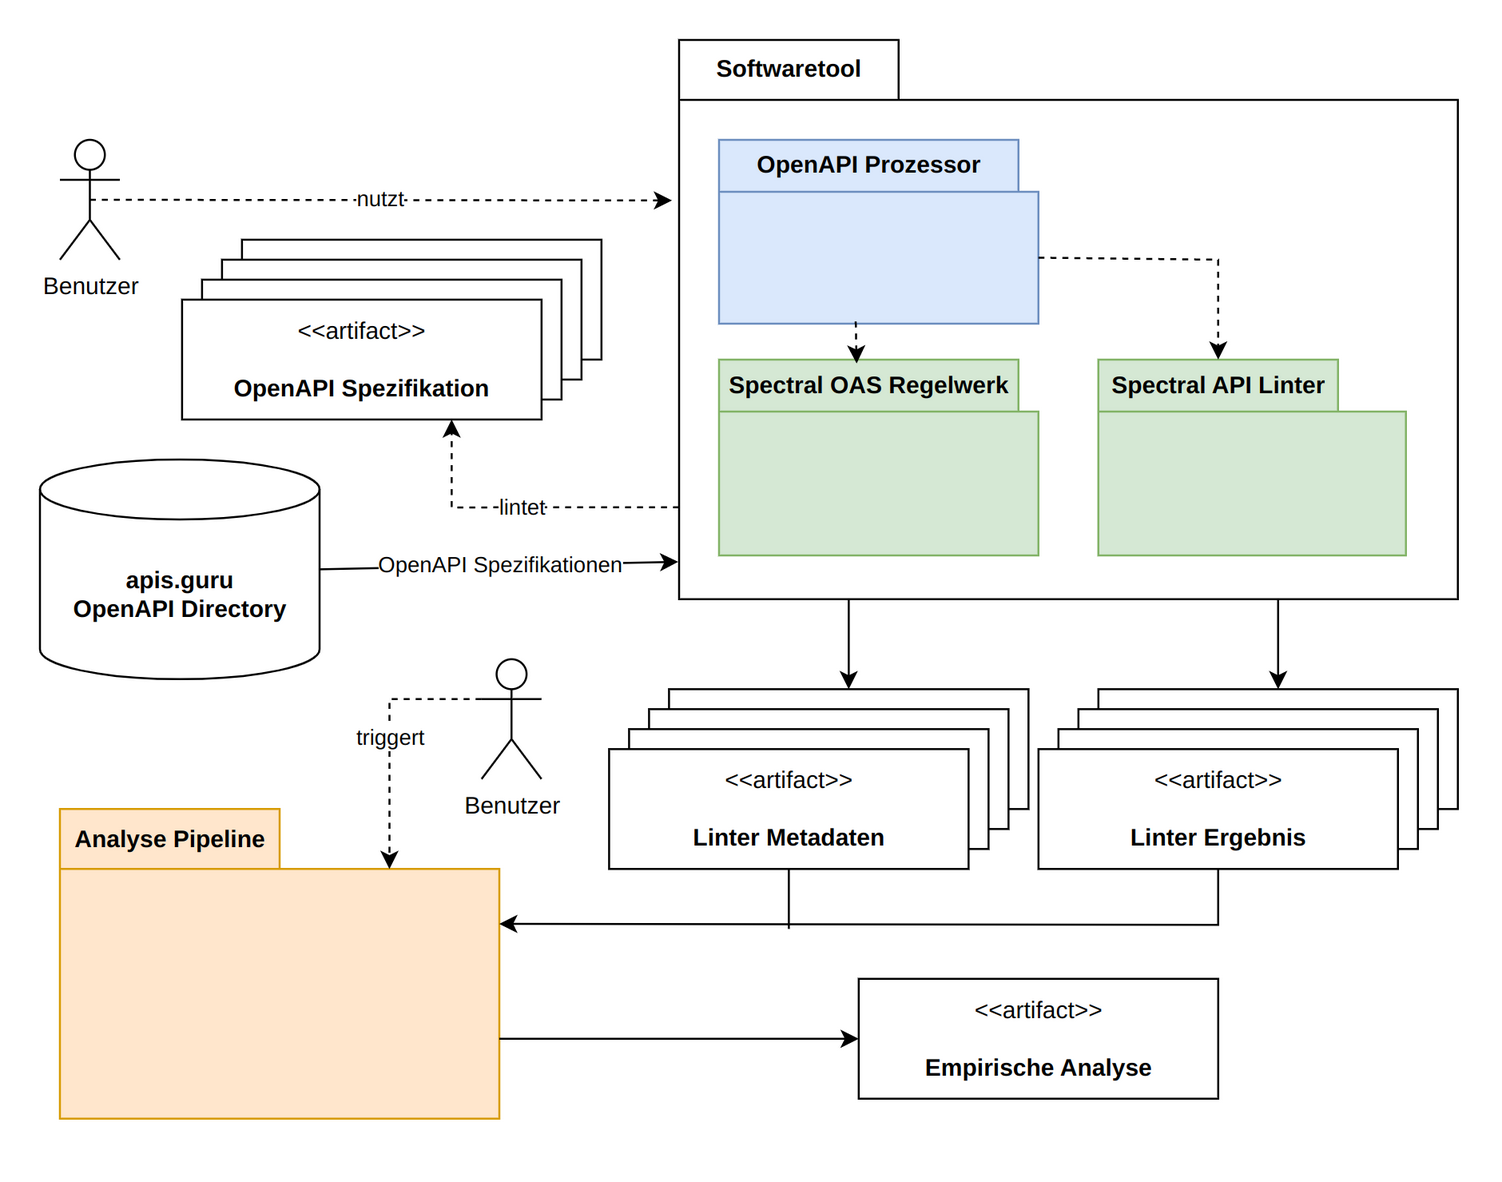
\includegraphics[width=1\linewidth]{img/contextview.png}
    \caption{Kontextsicht auf Architektur des zu entwickelnden Softwaretools}
    \label{fig:Kontextsicht}
\end{figure}

Ein Use Case für das System könnte der folgende sein:

\textbf{Einlesen von OpenAPI Spezifikationen}

\begin{itemize}
    \item \textbf{System:} OpenAPI Ruleset Evaluator
    \item \textbf{Use Case:} 1
    \item \textbf{Akteur:} USER
    \item \textbf{Flow:} Ein User übergibt eine Liste von OpenAPI Spezifikationen an das System. Die Spezifikationen können sowohl als Liste einzelner Pfade zu Dateien, als auch in Form eines Ordners übergeben werden.
    \item \textbf{Nachbedingung:} Das System speichert die Pfade zu den OpenAPI Spezifikationen
    \item \textbf{Qualitätsanforderungen:}
    \begin{itemize}
        \item Der angegebene Flow kann erfolgreich ausgeführt werden (Funktionalität)
        \item Es werden nur valide OpenAPI Spezifikationen angenommen (Funktionalität)
        \item Es werden nur gültige Pfade angenommen (Funktionalität)
        \item Die Eingabe erfolgt über ein CLI Tool (Benutzbarkeit)
    \end{itemize}
\end{itemize}

Daraus leiten sich dann die tatsächlichen Implikationen zur Implementierung als User Storys und Akzeptanzkriterien ab. User Storys für die Implementierungsphase, werden in einem separaten Backlog gesammelt. In der Implementierungsphase werden diese abgearbeitet und der Arbeitsfluss wird mithilfe von \textit{To-do}, \textit{in Progress} und \textit{Done} Status der Storys dokumentiert.

Außerdem sollen Qualitätsanforderungen gesammelt werden, die Funktionalität, Effizienz, Kompatibilität, Benutzbarkeit, Zuverlässigkeit, Sicherheit, Wartbarkeit und Portierbarkeit des zu entwickelnden Tools definieren. Letztendlich sollen auch Einschränkungen erkannt werden. Eine Einschränkung wird hier beispielhaft genannt:

\begin{itemize}
    \item Um alle Features des API Linter Tools Spectral nutzen zu können, muss das Tool in NodeJS entwickelt werden.
\end{itemize}

Weiterhin sollen die ermittelten Daten empirisch analysiert werden. Dazu zählen die Datenvorverarbeitung, wie zum Beispiel das Umformen von Rohdaten in eine Tabelle. Zum Extrahieren von Informationen zählt  auch das Invertieren der Ergebnisse, um anstelle von Informationen zu Linterfehlern, Informationen über das erfolgreiche Einhalten von Linterregeln zu erhalten. In einer explorativen Datenanalyse sollen verschiedene Methoden angewendet werden, um die Verteilung der Daten zu beschreiben. Dazu gehört ein Boxplot über die Linterregeln, in dem die Verteilung der Linterfehler visualisiert wird. Zum Ermitteln von Trends und Gruppierungen sollen hierarchische Cluster-Verfahren verwendet werden.

Mit der Sicherstellung der Qualität der Daten\footnote{Mehr dazu unter Evaluierungsstrategie}, wird davon ausgegangen, dass Linterregeln, die Fehler ausgelöst haben, keine Auswirkung auf Qualität der OpenAPI Spezifikationen haben. Diese Annahme ermöglicht, die Relevanz einer Linterregel mit den erfolgreichen Einhaltungen im Datensatz gleichzusetzen. Mit dieser Annahme sollen die Ergebnisse interpretiert werden. Anhand der charakteristischen Werte für jede Linterregel können Aussagen über Relevanz und Priorisierung getroffen werden.




\section{Evaluierungsstrategie}
Um von Beginn an die Methodik zu evaluieren und wissenschaftlich zu arbeiten, werden verschiedene Maßnahmen ergriffen.

Für die Argumentation der Thesis ist es wichtig, die Qualität der verwendeten Daten sicherzustellen.
Dies ist möglich, indem wissenschaftliche Artikel referenziert werden, die diesen Datensatz verwenden. Für das Jahr 2024 gibt es mindestens drei Artikel eines verwandten Themengebietes, die das apis.guru OpenAPI Directory verwenden \parencite{bogner_restruler_2024}\parencite{serbout_apistic_2024}\parencite{kim_leveraging_2024}. In \parencite{serbout_apistic_2024} wird die hohe Qualität der Daten des apis.guru Datensatzes wie folgt begründet: \textit{„[...] because of its curated content it contains
high-quality, valid and distinct specifications as „non-reliable“ APIs
are filtered out.“}. Trotzdem sollen in der Arbeit durch Verwendung des Datensatzes entstehende Risiken untersucht werden.

Auch in der empirischen Analyse werden Methoden zum Verifizieren der Ergebnisse eingesetzt. Dazu gehört, die ermittelten Cluster und Gruppen zu evaluieren. Es soll beispielsweise der Silhouetten-Koeffizient angewendet werden, der zeigt, wie passend die Clustereinteilung ist.

Weiterhin sollen Methoden zur Qualitätssicherung des Softwaretools eingesetzt werden:
\begin{itemize}
    \item Der geschriebene Code wird in TDD (Test Driven Development) entwickelt.
    \item Es soll ein Quality Gate von 80 \% Testabdeckung für den entwickelten Programmcode festgelegt werden.
\end{itemize}

\section{Kontext}
Die Bachelorarbeit wird in Zusammenarbeit mit dem Unternehmen SAP LeanIX durchgeführt. Im Rahmen eines Praxisprojekts im Herbst 2023 wurden dort verschiedene Softwaretools für das Linten von OpenAPI Spezifikationen anhand interner Guidelines untersucht. Aus den Erkenntnissen des Praxisprojekts lässt sich das anfängliche Problem herleiten.

SAP LeanIX ist einer der führenden Enterprise Architecture Management (EAM) Lösungen. Die SAP LeanIX EAM Software ist eine datengetriebene und auf Zusammenarbeit ausgerichtete Lösung, die Enterprise Architekten bei der Organisation und Verwaltung von der eingesetzten Software des Unternehmens und deren internen Abhängigkeiten, sowie bei der Planung von Zukunftsarchitekturen unterstützt. 
LeanIX setzt bei der Produktentwicklung auf eine Mikroservicearchitektur. Die Services nutzen verschiedene Technologien und stellen im Allgemeinen REST APIs zum Informationsaustausch zur Verfügung, die mithilfe von OpenAPI öffentlich dokumentiert werden.


\section{Gliederungsentwurf}
\begin{enumerate}[label*=\arabic*.]
    \item Einleitung
    \begin{enumerate}[label*=\arabic*.]
        \item Problem Statement
        \item Forschungsfragen
        \item Mehrwert und Motiv
        \item Methode
        \item Struktur
    \end{enumerate}
    \item Forschungsstand
    \begin{enumerate}[label*=\arabic*.]
        \item REST APIs
        \begin{enumerate}[label*=\arabic*.]
            \item Geschichte
            \item Umsetzung Http und URI
            \item Qualitätskriterien
        \end{enumerate}
        \item OpenAPI
        \item Linter
        \begin{enumerate}[label*=\arabic*.]
            \item Tools
            \item Spectral
            \item OAS Regelwerk
        \end{enumerate}
        \item Related Work
    \end{enumerate}
    \item Herleitung der Methode
    \begin{enumerate}[label*=\arabic*.]
        \item Verwendeter Datensatz
        \item Anforderungsermittlung
        \item Konzeption
        \item Implementierung
        \item Datenaufbereitung
                \begin{enumerate}[label*=\arabic*.]
            \item Invertierung
        \end{enumerate}
        \item Datenanalyse
    \end{enumerate}
    \item Anwenden der Methode
    \begin{enumerate}[label*=\arabic*.]
        \item Codeausführung
    \end{enumerate}
    \item Ergebnisse und Analyse
    \begin{enumerate}[label*=\arabic*.]
        \item Explorative Analyse
        \begin{enumerate}[label*=\arabic*.]
            \item Deskriptive Statistik
            \item Verteilungen
            \item Clusteranalyse
        \end{enumerate}
        \item Mapping zu Relevanz (RQ1)
        \begin{enumerate}[label*=\arabic*.]
            \item Priorisieren der Linterregeln (RQ2)
            \item Empfehlung von Linterregeln (RQ3)
        \end{enumerate}
    \end{enumerate}
    \item Evaluation
    \begin{enumerate}[label*=\arabic*.]
        \item Abgleich mit Methode
        \item Validität des Verfahrens
        \item Risiken
    \end{enumerate}
    \item Ausblick
    \item Literaturverzeichnis
    \item Anhang
\end{enumerate}

\section{Zeitplan}

\vspace{.5cm}
\definecolor{confcol1}{RGB}{159, 143, 239}
\definecolor{confcol2}{RGB}{223, 216, 253}
\definecolor{confcol3}{RGB}{243, 240, 255}
\definecolor{confcol4}{RGB}{255, 213, 210}
\definecolor{confcol5}{RGB}{255, 236, 235}
\definecolor{confcol6}{RGB}{248, 230, 160}
\definecolor{confcol7}{RGB}{255, 247, 214}
\definecolor{confcol8}{RGB}{220, 255, 241}
\definecolor{confcol9}{RGB}{185, 243, 219}
\definecolor{confcol10}{RGB}{73, 197, 146}

\begin{ganttchart}[
    vgrid,
    %hgrid,
    x unit=0.7cm,
    y unit title=0.6cm,
    y unit chart=0.6cm,
    title/.append style={fill=gray!10},
    title label font=\bfseries,
    title height=1,
    bar height=0.7,
    bar/.append style={fill},
    bar incomplete/.append style={fill=blue!50},
    bar/.append style={fill=blue!50},
    progress label text={},
    milestone label font=\bfseries\small,
    milestone height=0.8,
    milestone top shift=0.2,
    milestone/.append style={fill=green},
    group/.append style={draw=black, fill=green!30},
    group height=.3,
    group peaks height=.2,
    group label font=\bfseries\small,
    group left shift=0,
    group right shift=0,
    group top shift=.3,
    group height=.2,
    group peaks tip position=0,
    group peaks width=0.2,
    group incomplete/.append style={fill=gray!50},
    link/.style={->,thick},
    expand chart=\textwidth,
    today=1,
    progress=0,
    %inline
    ]{1}{13}
    
    \gantttitle{Bachelorthesis}{13} \\
    \ganttbar{\textbf{Wochen}}{-20}{-20}
    \gantttitlelist{1,...,13}{1} \\
  
    \ganttbar[bar incomplete/.append style={fill=confcol1}]{Anforderungserhebung(S)}{1}{3} \\
    \ganttbar[bar incomplete/.append style={fill=confcol2}]{Forschungsstand(S)}{1}{4} \\
    \ganttbar[bar incomplete/.append style={fill=confcol3}]{Datensatz erstellen(P)}{3}{3} \\

    \ganttmilestone{Milestone 1}{4} \\
    
    \ganttbar[bar incomplete/.append style={fill=confcol4}]{Vorgehen dokumentieren(S)}{3}{6} \\
    \ganttbar[bar incomplete/.append style={fill=confcol5}]{Konzeption(S)}{4}{5} \\
    \ganttbar[bar incomplete/.append style={fill=confcol6}]{Entwicklung(P)}{5}{8} \\
    \ganttbar[bar incomplete/.append style={fill=confcol7}]{Empirische Analyse(P)}{7}{9} \\

    \ganttmilestone{Milestone 2}{10} \\

    \ganttbar[bar incomplete/.append style={fill=confcol8}]{Ergebnisse dokumentieren(S)}{8}{11} \\
    \ganttbar[bar incomplete/.append style={fill=confcol9}]{Ergebnisse interpretieren(S)}        {9}{11} \\
    \ganttbar[bar incomplete/.append style={fill=confcol10}]{Finalisieren(S)}                    {11}{13} \\
    

\end{ganttchart}

\begin{itemize}
    \item (P) - Programmieren
    \item (S) - Schreiben
\end{itemize}

\textbf{Milestones:}
\begin{itemize}
    \item Milestone 1: Anforderungserhebung und Schreiben des Forschungsstandes sind abgeschlossen.
    \item Milestone 2: Alle Programmiertasks sind abgeschlossen. Die verbleibenden Aufgaben sind ausschließlich Schreibtasks.
\end{itemize}